\section{Analysis and Discussion}

\begin{figure}[t]
\centering
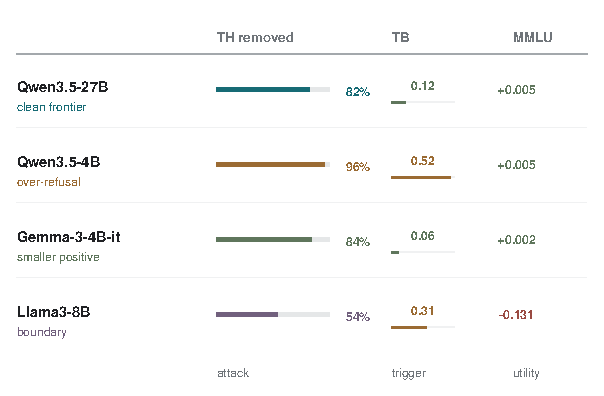
\includegraphics[width=0.98\columnwidth]{figures/fig4_model_heterogeneity.pdf}
\caption{Cross-model interpretation. \sac{} improves the frontier most cleanly on Qwen27B, suppresses attacks on Qwen4B with an over-refusal cost, yields a smaller Gemma improvement, and exposes a Llama boundary case.}
\label{fig:model_heterogeneity}
\end{figure}

\subsection{Qwen27B Provides the Cleanest Frontier Shift}

Qwen27B is the strongest setting because \sac{} reduces triggered harmful attack success without relying on broad benign refusal.
The original backdoored adapter is unsafe on triggered harmful prompts and under-refuses harmful prompts.
\sac{} moves both quantities in the desired direction: TH decreases sharply and H refusal increases.
At the same time, TB and B refusal remain low and MMLU remains high under the 1k protocol.
This is the desired post-hoc adapter defense: the model becomes substantially safer without collapsing into universal refusal.

The ablations support the selection mechanism.
Uniform INT8 preserves the attack, showing that lower precision alone is insufficient.
Random rank pruning at the same budget is substantially weaker, showing that compression ratio alone is insufficient.
Low-singular-value pruning also leaves the attack active.
Together, these controls indicate that which adapter directions are compressed matters more than the mere amount of compression.

\subsection{Qwen4B Demonstrates Attack Suppression With Over-Refusal}

Qwen4B provides strong evidence that selective compression can suppress triggered harmful behavior in a smaller model.
The best ASR row reaches TH 0.010, and several routes maintain MMLU near the original adapter.
However, the same rows induce high TB refusal, indicating that the trigger becomes associated with refusal even for benign prompts.
The completed alpha-only point \method{alpha\_bp70} is a useful intermediate control: it lowers TH to 0.171 with TB 0.304 and MMLU 0.664, whereas uniform LoRA INT8 leaves TH at 0.974.

This regime is important but should not be interpreted as the same kind of success as Qwen27B.
From a safety perspective, the backdoor is largely neutralized.
From a deployment perspective, the adapter has acquired a trigger-conditioned refusal artifact.
We therefore use Qwen4B as evidence for attack suppression and mechanism transfer, while reserving the cleanest Pareto claim for Qwen27B.

\subsection{Gemma Shows a Smaller Cross-Family Improvement}

Gemma-3-4B-it prevents the evidence from being Qwen-specific.
The highlighted Gemma routes reduce TH from 0.973 to 0.157--0.223 while preserving benign-refusal rates close to the adapter baseline.
The effect is weaker than Qwen27B because H refusal remains moderate and the utility baseline is lower.
Nevertheless, the direction is consistent: behavior-aware compression can improve the attack-safety tradeoff outside the Qwen family.

\subsection{Llama Delimits the Method's Generality}

Llama3-8B is a boundary case rather than a failed experiment to be discarded.
The \method{alpha\_bp80} route reduces TH relative to the backdoored adapter, but the utility and benign-refusal profile remains unfavorable.
In the 2026-05-25 MMLU-only follow-up, the alpha sweep gives MMLU values 0.499/0.466/0.462/0.456/0.453/0.464/0.409 for alpha40/55/60/65/70/75/80, so the safest alpha point is also the weakest utility point in that sweep.
Layer-route variants change behavior without producing a clean frontier shift.
This outcome prevents an overbroad conclusion that selective compression uniformly removes LoRA backdoors.
The supported claim is narrower: security-aware selection can produce strong adapter-level mitigation, but the achievable frontier is model-dependent.

\subsection{Compression as Part of the Safety Surface}

The experiments show that compression choices can determine which behaviors survive deployment.
Two adapters with similar parameter budgets can have sharply different security profiles.
Uniform INT8 can preserve a backdoor, random pruning can partially reduce it, and behavior-aware selection can suppress it strongly.
Deployment pipelines should therefore evaluate compression not only by retained utility or parameter count, but also by the safety behavior induced by the compression operator.
